% questions.tex —— 2003 年·全国新课程卷·文科 · 题目内容片段（无答案）
% 由 tools/generate_projects.py 依来源总账自 2003/2003_数学真题_全国新课程文_试题.md 生成，勿手改（改源 MD 后重跑）


\gkpart{数学}

\begin{gktip}
\textbf{来源说明}：本题面依据固定源 PDF 两页 A3 题面逐题转录，原卷印刷页码 144–145。固定源不附答案，答案和解析均由本库独立复算。

\textbf{图形说明}：第 17、18、22 题的原卷图形关系重绘为 TikZ/PGFPlots 矢量图。图形标记所指的 PNG 不随仓库保存。
\end{gktip}

\gkpart{一、选择题}

\begin{question}
\gkti{1}不等式 $\sqrt{4x-x^2}<x$ 的解集是\mbox{（　　）}

（A）$(0,2)$　　（B）$(2,+\infty)$　　（C）$(2,4)$　　（D）$(-\infty,0)\cup(2,+\infty)$

\end{question}
\begin{question}
\gkti{2}已知 $x\in\left(-\dfrac\pi2,0\right)$，$\cos x=\dfrac45$，则 $\tan2x=$\mbox{（　　）}

（A）$\dfrac7{24}$　　（B）$-\dfrac7{24}$　　（C）$\dfrac{24}{7}$　　（D）$-\dfrac{24}{7}$

\end{question}
\begin{question}
\gkti{3}

\nopagebreak[4]
\[
\frac{1-\sqrt3 i}{(\sqrt3+i)^2}
\]

的值为\mbox{（　　）}

（A）$\dfrac14+\dfrac{\sqrt3}{4}i$　　（B）$-\dfrac14-\dfrac{\sqrt3}{4}i$

（C）$\dfrac12+\dfrac{\sqrt3}{2}i$　　（D）$-\dfrac12-\dfrac{\sqrt3}{2}i$

\end{question}
\begin{question}
\gkti{4}已知 $x\in\left(-\dfrac\pi2,0\right)$，$\cos x=\dfrac45$，则 $\tan2x=$\mbox{（　　）}

（A）$\dfrac7{24}$　　（B）$-\dfrac7{24}$　　（C）$\dfrac{24}{7}$　　（D）$-\dfrac{24}{7}$

\end{question}
\begin{question}
\gkti{5}等差数列 $\{a_n\}$ 中，已知 $a_1=\dfrac13$，$a_2+a_5=4$，$a_n=33$，则 $n$ 为\mbox{（　　）}

（A）48　　（B）49　　（C）50　　（D）51

\end{question}
\begin{question}
\gkti{6}双曲线虚轴的一个端点为 $M$，两个焦点为 $F_1\text{、}F_2$，$\angle F_1MF_2=120^\circ$，则双曲线的离心率为\mbox{（　　）}

（A）$\sqrt3$　　（B）$\dfrac{\sqrt6}{2}$　　（C）$\dfrac{\sqrt6}{3}$　　（D）$\dfrac{\sqrt3}{3}$

\end{question}
\begin{question}
\gkti{7}设函数

\nopagebreak[4]
\[
f(x)=
\begin{cases}
2^{-x}-1,&x\leqslant0,\\
x^2,&x>0,
\end{cases}
\]

若 $f(x_0)>1$，则 $x_0$ 的取值范围是\mbox{（　　）}

（A）$(-1,1)$　　（B）$(-1,+\infty)$

（C）$(-\infty,-2)\cup(0,+\infty)$　　（D）$(-\infty,-1)\cup(1,+\infty)$

\end{question}
\begin{question}
\gkti{8}$O$ 是平面上一定点，$A\text{、}B\text{、}C$ 是平面上不共线的三个点，动点 $P$ 满足

\nopagebreak[4]
\[
\overrightarrow{OP}
=\overrightarrow{OA}
+\lambda\left(
\frac{\overrightarrow{AB}}{|\overrightarrow{AB}|}
+\frac{\overrightarrow{AC}}{|\overrightarrow{AC}|}
\right),\qquad \lambda\in[0,+\infty),
\]

则 $P$ 的轨迹一定通过 $\triangle ABC$ 的\mbox{（　　）}

（A）外心　　（B）内心　　（C）重心　　（D）垂心

\end{question}
\begin{question}
\gkti{9}函数

\nopagebreak[4]
\[
y=\ln\frac{x+1}{x-1},\qquad x\in(1,+\infty)
\]

的反函数为\mbox{（　　）}

（A）$y=\dfrac{e^x-1}{e^x+1},\ x\in(0,+\infty)$

（B）$y=\dfrac{e^x+1}{e^x-1},\ x\in(0,+\infty)$

（C）$y=\dfrac{e^x-1}{e^x+1},\ x\in(-\infty,0)$

（D）$y=\dfrac{e^x+1}{e^x-1},\ x\in(-\infty,0)$

\end{question}
\begin{question}
\gkti{10}棱长为 $a$ 的正方体中，连接相邻面的中心，以这些线段为棱的八面体的体积为\mbox{（　　）}

（A）$\dfrac{a^3}{3}$　　（B）$\dfrac{a^3}{4}$　　（C）$\dfrac{a^3}{6}$　　（D）$\dfrac{a^3}{12}$

\end{question}
\begin{question}
\gkti{11}设 $a>0$，$f(x)=ax^2+bx+c$，曲线 $y=f(x)$ 在点 $P(x_0,f(x_0))$ 处切线的倾斜角的取值范围为 $\left[0,\dfrac\pi4\right]$，则 $P$ 到曲线 $y=f(x)$ 对称轴距离的取值范围为\mbox{（　　）}

（A）$\left[0,\dfrac1a\right]$　　（B）$\left[0,\dfrac1{2a}\right]$　　（C）$\left[0,\dfrac{|b|}{2a}\right]$　　（D）$\left[0,\dfrac{|b-1|}{2a}\right]$

\end{question}
\begin{question}
\gkti{12}已知长方形的四个顶点 $A(0,0)\text{、}B(2,0)\text{、}C(2,1)\text{、}D(0,1)$，一质点从 $AB$ 的中点 $P_0$ 沿与 $AB$ 的夹角为 $\theta$ 的方向射到 $BC$ 上的点 $P_1$ 后，依次反射到 $CD\text{、}DA$ 和 $AB$ 上的点 $P_2\text{、}P_3$ 和 $P_4$（入射角等于反射角）。设 $P_4$ 的坐标为 $(x_4,0)$，若 $1<x_4<2$，则 $\tan\theta$ 的取值范围是\mbox{（　　）}

（A）$\left(\dfrac13,1\right)$　　（B）$\left(\dfrac13,\dfrac23\right)$　　（C）$\left(\dfrac25,\dfrac12\right)$　　（D）$\left(\dfrac25,\dfrac23\right)$

\end{question}
\begin{question}
\gkti{13}一个四面体的所有棱长都为 $\sqrt2$，四个顶点在同一球面上，则此球的表面积为\mbox{（　　）}

（A）$3\pi$　　（B）$4\pi$　　（C）$3\sqrt3\pi$　　（D）$6\pi$

\end{question}
\gkpart{二、填空题}

\begin{question}
\gkti{14}$\left(x^2-\dfrac1{2x}\right)^9$ 的展开式中 $x^9$ 的系数是\gkblank{}。

\end{question}
\begin{question}
\gkti{15}某公司生产三种型号的轿车，产量分别为 1200 辆、6000 辆和 2000 辆。为检验该公司的产品质量，现用分层抽样的方法抽取 46 辆进行检验，这三种型号的轿车依次应抽取\gkblank{}、\gkblank{}、\gkblank{}辆。

\end{question}
\begin{question}
\gkti{16}在平面几何里，有勾股定理：“设 $\triangle ABC$ 的两边 $AB\text{、}AC$ 互相垂直，则 $AB^2+AC^2=BC^2$。”拓展到空间，类比平面几何的勾股定理，研究三棱锥的侧面面积与底面面积间的关系，可以得出的正确结论是：“设三棱锥 $A-BCD$ 的三个侧面 $ABC\text{、}ACD\text{、}ADB$ 两两互相垂直，则\gkblank{}。”

\Needspace{0.4\textheight}
\end{question}
\begin{question}
\gkti{17}将 3 种作物种植在如图 5 块试验田里，每块种植一种作物且相邻的试验田不能种植同一作物，不同的种植方法共有\gkblank{}种。（以数字作答）
\nopagebreak[4]
\begin{center}% 2003 年全国新课程文科第 17 题：五块试验田
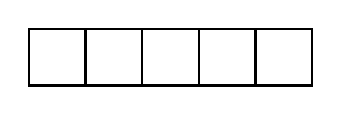
\begin{tikzpicture}[scale=0.72]
  \draw[thick] (0,0) rectangle (5,1);
  \foreach \x in {1,2,3,4} \draw[thick] (\x,0)--(\x,1);
\end{tikzpicture}
\end{center}
\nopagebreak[4]
\end{question}
\gkpart{三、解答题}

\Needspace{0.4\textheight}
\begin{question}
\gkti{18}已知正四棱柱 $ABCD-A_1B_1C_1D_1$，$AB=1$，$AA_1=2$，$E$ 为 $CC_1$ 中点，$F$ 为 $BD_1$ 中点。
\nopagebreak[4]
\begin{center}% 2003 年全国新课程文科第 18 题：正四棱柱
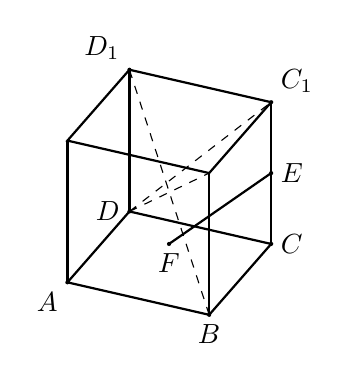
\begin{tikzpicture}[>=stealth,scale=0.75]
  \coordinate (A) at (0,0); \coordinate (B) at (2.4,-0.55);
  \coordinate (C) at (3.45,0.65); \coordinate (D) at (1.05,1.2);
  \coordinate (A1) at (0,2.4); \coordinate (B1) at (2.4,1.85);
  \coordinate (C1) at (3.45,3.05); \coordinate (D1) at (1.05,3.6);
  \coordinate (E) at (3.45,1.85); \coordinate (F) at (1.72,0.65);
  \draw[thick] (A)--(B)--(C)--(D)--cycle;
  \draw[thick] (A1)--(B1)--(C1)--(D1)--cycle;
  \draw[thick] (A)--(A1) (B)--(B1) (C)--(C1) (D)--(D1);
  \draw[dashed] (B)--(D1) (D)--(B1) (D)--(C1);
  \draw[thick] (E)--(F);
  \fill (A) circle (1pt) node[below left] {$A$};
  \fill (B) circle (1pt) node[below] {$B$};
  \fill (C) circle (1pt) node[right] {$C$};
  \fill (D) circle (1pt) node[left] {$D$};
  \fill (D1) circle (1pt) node[above left] {$D_1$};
  \fill (C1) circle (1pt) node[above right] {$C_1$};
  \fill (E) circle (1pt) node[right] {$E$};
  \fill (F) circle (1pt) node[below] {$F$};
\end{tikzpicture}
\end{center}
\nopagebreak[4]
（1） 证明：$EF$ 为 $BD_1$ 与 $CC_1$ 的公垂线；

（2） 求点 $D_1$ 到面 $BDE$ 的距离。

\end{question}
\begin{question}
\gkti{19}已知抛物线 $C_1:y=x^2+2x$ 和 $C_2:y=-x^2+a$。如果直线 $l$ 同时是 $C_1$ 和 $C_2$ 的切线，称 $l$ 是 $C_1$ 和 $C_2$ 的公切线，公切线上两个切点之间的线段称为公切线段。

（1） $a$ 取什么值时，$C_1$ 和 $C_2$ 有且仅有一条公切线？写出此公切线的方程；

（2） 若 $C_1$ 和 $C_2$ 有两条公切线，证明相应的两条公切线段互相平分。

\end{question}
\begin{question}
\gkti{20}已知数列 $\{a_n\}$ 满足 $a_1=1$，$a_n=3^{n-1}+a_{n-1}$（$n\geqslant2$）。

（1） 求 $a_2\text{、}a_3$；

（2） 证明：$a_n=\dfrac{3^n-1}{2}$。

\end{question}
\begin{question}
\gkti{21}有三种产品，合格率分别为 $0.90\text{、}0.95\text{、}0.95$，各抽取一件进行检验。

（1） 求恰有一件不合格的概率；

（2） 求至少有两件不合格的概率（精确到 $0.001$）。

\Needspace{0.4\textheight}
\end{question}
\begin{question}
\gkti{22}已知函数

\nopagebreak[4]
\[
f(x)=\sin(\omega x+\varphi)\qquad(\omega>0,\ 0\leqslant\varphi\leqslant\pi)
\]

是 $\mathbb R$ 上的偶函数，其图象关于点 $M\left(\dfrac{3\pi}{4},0\right)$ 对称，且在区间 $\left[0,\dfrac\pi2\right]$ 上是单调函数，求 $\omega$ 和 $\varphi$ 的值。
\nopagebreak[4]
\begin{center}% 2003 年全国新课程文科第 22 题：正弦函数图象坐标系
\begin{tikzpicture}[x=1.0cm,y=0.7cm,>=stealth]
  \draw[->] (-1.9,0)--(1.9,0) node[right] {$x$};
  \draw[->] (0,-1.4)--(0,1.6) node[above] {$y$};
  \node[below] at (-1.57,0) {$-\frac\pi2$};
  \node[below] at (1.57,0) {$\frac\pi2$};
  \node[below left] at (0,0) {$O$};
\end{tikzpicture}
\end{center}
\nopagebreak[4]
\end{question}
\begin{question}
\gkti{23}已知常数 $a>0$，向量 $\vec c=(0,a)$，$\vec i=(1,0)$。经过原点 $O$ 以 $\vec c+\lambda\vec i$ 为方向向量的直线与经过定点 $A(0,a)$ 以 $\vec i-2\lambda\vec c$ 为方向向量的直线相交于 $P$，其中 $\lambda\in\mathbb R$。试问：是否存在两个定点 $E\text{、}F$，使得 $|PE|+|PF|$ 为定值？若存在，求出 $E\text{、}F$ 的坐标；若不存在，说明理由。

\end{question}